\documentclass[10pt]{mypackage}

% sans serif font:
%\usepackage{cmbright,sfmath,bbold}
%\renewcommand{\mathcal}{\mathtt}

%Euler:
\usepackage{newpxtext,eulerpx,eucal,eufrak}
\renewcommand*{\mathbb}[1]{\varmathbb{#1}}
\renewcommand*{\hbar}{\hslash}

\usepackage{homework}

\pagestyle{fancy} %better headers
\fancyhf{}
\rhead{Avinash Iyer}
\lhead{Math 401: Mathematical Problem Solving}

\setcounter{secnumdepth}{0}

\begin{document}
\RaggedRight
\section{Homework Problems}%
\begin{problem}[Homework Problem 1]
  Given an infinite chessboard where each tile is given a strictly positive integral value equal to the average of its four non-diagonal neighbors, must every square have the same value.
\end{problem}
\begin{solution}
  The answer is \textbf{yes}.\newline

  Suppose not. If not every square is the same value, then there must exist a pair of neighboring squares with unequal value. Call these squares $\mathbf{x_1}$ and $\mathbf{x_2}$, where $x_1 > x_2$. Here, $x_1,x_2$ refer to values, while $\mathbf{x_1},\mathbf{x_2}$ refer to the boxes.\newline

  Then, it must be the case that there is some neighbor $\mathbf{x_3}$ such that $x_3 < x_2$. Else, by the average rule, we have
  \begin{align*}
    x_2 &\geq \frac{x_2 + x_2 + x_2 + x_1}{4}\\
        &> x_2,
  \end{align*}
  which is a contradiction.\newline

  Via infinite descent, we continue finding boxes $\mathbf{x_{k}}$ such that $x_{k+1} < x_k$, implying that there are infinitely many boxes with integral value less than $x_1$.
\end{solution}
\begin{solution}[Alternative Solution]
  By the well-ordering principle, there is a smallest positive integer in the collection of squares. Let this be in the box $\mathbf{s}$ with value $s$. Then, neighbor of $\mathbf{s}$ must all have the same value, or else $s$ would not have the smallest value.
\end{solution}
\begin{problem}[Homework Problem 2]
Given $n+1$ bit strings of length $n$, where $n\geq 2$, if you can only ask questions of the form ``what is the value of bit $i$ in string $j$,'' determine the minimum number of questions you can ask to guarantee the construction of a string different from any of those $n+1$ strings.
\end{problem}
\begin{solution}
  The answer is $\mathbf{n+2}$.\newline

  For ease of notation, we will number the strings $1,\dots,n+1$, and let $v(j,i)$ yield the value of bit $i$ in string $j$.\newline

  Consider $S = \left(v\left(1,1\right),v\left(2,1\right),v\left(3,1\right)\right)$. By the pigeonhole principle, it is either case that at least two of the values in the tuple $S$ are either $0$ or $1$. Without loss of generality, let $v\left(1,1\right) = v\left(2,1\right) = 1$. Then, consider $S' = v\left(i+1,i\right)$ for bits $2 \leq i \leq n$.\newline

  We will construct the target bit string $t$ by starting with $0$, and if $t\left(i\right) = 1-v\left(i+1,i\right)$.\newline

  For $i\geq 3$, our target string $t$ disagrees with $s_i$ at position $i-1$, and our target string $t$ disagrees with both the first and second string at position $1$. This shows that we can find our target string in $n+2$ questions.\newline

  Now, we show that we cannot guarantee a divergent string in $n+1$ questions. Note that since there are $n$ coordinates, we cannot ask fewer than $n$ questions. On guess number $n+1$, we must ask a question about a coordinate that has already been guessed. If this coordinate is equal to one of the coordinates in our draft target string, then we need to ask at least one more question to be able to guarantee that our string is divergent.
\end{solution}
\begin{problem}[Homework Problem 3]
  Consider a set $\set{a_1,\dots,a_{n+1}}$ of positive integers such that all $a_i \leq 2n$. Show that there are $i,j$ such that $a_i | a_j$.
\end{problem}
\begin{solution}
  We may write the collection as $2^{e_1}x_1,\dots, 2^{e_{n+1}}x_{n+1}$, with all of $x_{1},\dots,x_{n+1}$ odd. Then, we have $x_1,\dots,x_{n+1}$ is a collection of $n+1$ odd numbers less than $2n$, so by the pigeonhole principle, we must have some $i,j$ such that $x_i = x_j$. Thus, without loss of generality, $2^{e_i}x_i | 2^{e_j}x_j$.
\end{solution}

\begin{problem}[Homework Problem 4]
Show that for every graph there is an orientation of the edges such that for every vertex the out-degree and in-degree differ by at most $1$.
\end{problem}
\begin{solution}
  Without loss of generality, we assume $G$ is connected. If $G$ is disconnected, we apply the following procedure to each of the connected components.\newline

  If all vertices in $G$ are of even degree, we may apply an orientation on $G$ by following an Eulerian circuit. Every vertex in this directed Eulerian circuit has degree zero.\newline

  If there are any vertices in $G$ of odd degree, we know that there must be an even number of these vertices of odd degree; call them $\set{v_1,\dots,v_{2n}}$. We add vertices $\set{w_1,\dots,w_n}$ and edges such that $w_i$ has an edge to $v_{2i-1}$ and $v_{2i}$. This new graph, call it $G'$, has an Eulerian circuit; we follow this Eulerian circuit to place an orientation on all edges. Since each $v_i$ has only one edge out to a $w_i$ (or one edge in from a $w_i$), we may delete $\set{w_1,\dots,w_n}$ to yield $G$ with an orientation of all edges that has difference at most one between in-degree and out-degree.
\end{solution}
\begin{problem}[Homework Problem 6]
Can you subdivide a cube into finitely many smaller cubes, no two of which have the same size.
\end{problem}
\begin{solution}
  The answer is no.\newline

  Suppose it is possible to do so. Then, the bottom face is can be split into smaller squares, no two of which have the same side length.\newline

  We claim that the smallest square is not on the edge of the bottom face. If the smallest square were on the edge, then it would necessitate another square of the same side length.\newline

  We have shown that the smallest square, $\square_m$, is somewhere in the interior of the bottom face.\newline

  Going back into three dimensions, we now see that the cube corresponding to the smallest square, is fully surrounded by larger cubes, all of which share the face with $\square_m$. The top of the cube corresponding to $\square_m$ is a square of size $\square_m$, meaning that $\square_m$ must be tiled with smaller squares. Thus, there is no smallest cube.
\end{solution}

\begin{problem}[Homework Problem 7]
Given 5 points in $\R^3$, show that there exists a closed half-space $H$ with $O = (0,0,0)\in \partial H$ such that $H$ contains at least four points.
\end{problem}
\begin{solution}
  Let $\set{p_1,p_2,p_3,p_4,p_5}$. If all five points are collinear, then select any plane passing through the points, and translate the plane to the origin.\newline

  Else, consider the plane formed by, without loss of generality, $p_1,p_2,O$. Then, by the pigeonhole principle, at least two of $p_3,p_4,p_5$ are on one side of this plane. This yields the four desired points.
\end{solution}
\begin{problem}[Homework Problem 9]
For convex subsets $C_1,\dots,C_n\subseteq \R^2$, if for all $i,j,k$ $C_i\cap C_j \cap C_k \neq \emptyset$, then
\begin{align*}
  \bigcap_{i=1}^{n}C_i\neq \emptyset.
\end{align*}
\end{problem}
\begin{solution}
  We start by showing that any $4$ of the sets have nonempty intersection.\newline

  Let $A,B,C,D\in \set{C_1,\dots,C_n}$. Let $DAB \in D\cap A \cap B$, and similarly $DAC$ and $DBC$. Let $H = \operatorname{conv}\left( DAB,DAC,DBC \right)$. If $ABC\in A\cap B \cap C$ is also an element of $H$, then we are done, since $H\subseteq D$.\newline

  Now, if $ABC\notin \mathcal{H}$, we consider the convex hull of our four points, $DAB,DBC,ABC,DAC$. Then, there are four possibilities:
  \begin{itemize}
    \item If our convex hull is a quadrilateral, then the intersection of the diagonals of the quadrilateral is in all four sets.
    \item If our convex hull is a triangle, then one of the elements $DAB,DBC,DAC,ABC$ is in all four sets.
    \item If our convex hull is a line, then one of the points in between all four of $DAB,DBC,DAC,ABC$' is in all four points.
    \item If our convex hull is a point, we are done.
  \end{itemize}
  In the case for $n > 4$, we use the procedure for the case of $4$ on each subset of four.
\end{solution}


\begin{problem}[Homework Problem 11]
  A set of integers $S$ is called sum-free if for any $x,y\in S$, $x+y\notin S$. Show that every set of $n\geq 1$ of nonzero integers has a sum-free subset of at least $n\geq 3$.
\end{problem}
\begin{solution}
  Let $A\subseteq \Z\setminus \set{0}$ be such that $\left\vert A \right\vert = n$. Let $p$ be a prime be such that $p > \max\set{\left\vert a \right\vert | a\in A}$. A set is sum-free if it sum-free modulo $p$.\newline

  Now, for all $a\in \left( \Z/p\Z \right)^{\times}$, we define $f_a\colon \Z/p\Z\rightarrow \Z/p\Z$ by $x\mapsto xa$. We know that $f_a$ is injective.\newline

  Find $p$ such that $p = 3k + 2$ and $p > \max\set{\left\vert a \right\vert | a\in A}$.\newline

  We note that $B = \set{k+1,\dots,2k+1}$ is sum-free modulo $p$ and has size $k + 1$, as $\left( k+1 \right) + \left( k+1 \right) = 2k + 2$ modulo $p$, and that $\left( 2k+1 \right) + \left( 2k+1 \right) = 4k + 2 \equiv k$ modulo $p$.\newline

  Let $x\in \left( \Z/p\Z \right)^{\times}$ be taken uniformly at random, and let $a\in A$. The probability that $f_a(x) \in B$ is $\frac{\left\vert B \right\vert}{p-1}$, or $\frac{k+1}{3k+1} > \frac{1}{3}$.\newline

  We have that the expected value of the number of $a\in A$ such that $f_a(x)\in B$ is $\sum_{a\in A}P\left( f_a(x)\in B \right)$. We define
  \begin{align*}
    I_a(x) &= \begin{cases}
      1 & f_a(x)\in B\\
      0 & \text{else}
    \end{cases}.
  \end{align*}
  Then, we have
  \begin{align*}
    E\left( I_a(x) \right) &= \sum_{a\in A}P\left( f_a(x)\in B \right)\\
                           &= P\left( f_a(x)\in b \right)\\
                           &= \frac{k+1}{3k+1}.
  \end{align*}
  
\end{solution}
%\begin{problem}[Homework Problem 13]
%An odd number of people are standing in a room. Each person shoots water at the person closest to them. Determine if one or neither of the following is true.
%\begin{enumerate}[(a)]
%  \item At least one person will not get wet.
%  \item Everyone will get wet.
%\end{enumerate}
%\end{problem}
%\begin{solution}
%  Let $x_1,\dots,x_{2k+1}$ be the people in the room. We will prove (a) --- that is, at last one person will not get wet.\newline
%
%  We start by claiming that there are no cycles. Letting $y_k$ be the distance between $x_{k}$ and $x_{k+1}$, where $y_{2k+1}$ denotes the distance between $x_{2k+1}$ and $x_1$.
%\end{solution}

\begin{problem}[Homework Problem 14]
  Is it possible to fit a box $X$ with sides $x_1,x_2,x_3$ into a box with sides $y_1,y_2,y_3$ such that $x_1 + x_2 + x_3 > y_1 + y_2 + y_3$?
\end{problem}
\begin{solution}
  The answer is \textbf{no}.\newline

  Note that if $X\subseteq Y$, then $\operatorname{diam}\left( X \right) \leq \operatorname{diam}\left( Y \right)$, where $\operatorname{diam}\left( X \right)$ denotes the length of the longest diagonal of the box $X$.\newline

  For a box, the diameter of the box (as a set) is the square root of $x_1^2 + x_2^2 + x_3^2$. Thus, we have
  \begin{align*}
    x_1^2 + x_2^2 + x_3^2 &\leq y_1^2 + y_2^2 + y_3^2.
  \end{align*}
  Now, we will show that the surface area of $X$ is less than or equal to the surface area of $Y$. This is because, placing the box $X$ into $Y$, we may project $Y$ onto any face of $X$, meaning that the surface area of the preimage of the projection of $Y$ onto a face of $X$ is greater than or equal to the area of the face of $X$.\newline

  Thus, since
  \begin{align*}
    \left( x_1 + x_2 + x_3 \right)^2 &= \operatorname{diam}\left( X \right)^2 + S(X)\\
                                     &\leq \operatorname{diam}\left( Y \right)^2 + S(Y)\\
                                     &= \left( y_1 + y_2 + y_3 \right)^2,
  \end{align*}
  we have that the linear size of $X$ cannot be bigger than the linear size of $Y$.
\end{solution}
\begin{problem}[Homework Problem 16]
Is there an uncountable set of subsets of $\N$ with pairwise finite intersections?
\end{problem}
\begin{solution}
  The answer is \textbf{yes}.\newline

  By the Cauchy construction of the real numbers, we know that any real number $r\in \R$ is equal to an equivalence class of Cauchy sequences of rational numbers, $\left( r_n \right)_n\subseteq \R$ such that $\left( r_n \right)_n\rightarrow r$.\newline

  Furthermore, for any two sequences $\left( s_n \right)_n$ and $\left( t_n \right)_n$ such that $\left( s_n \right)_n\rightarrow s$ and $\left( t_n \right)_n\rightarrow t$,  if (without loss of generality) $s > t$, then there is some $\ve > 0$ such that $s - \ve > t + \ve$ (as $\R$ is Hausdorff), and by the definition of convergence, there is some $N$ such that for all $n\geq N$, $\left\vert s_n - s \right\vert < \ve$ and $\left\vert t_n - t \right\vert < \ve$, implying that $t_n\neq s_n$ for all $n\geq N$. Thus, we know that any two such sequences that converge to different values in $\R$ can only have a finite intersection.\newline

  Enumerating $\Q $ by taking $ \set{q_k}_{k\in \Q} = \N$, we select one representative equivalence class from each Cauchy sequence $\left( r_n \right)_n\rightarrow r$ for each $r\in R$, and define $S_r \coloneq \set{q_{r_n}}\subseteq \N$. Then, since each representative converges to a different real number $r\in \R$, any two such representatives can only have pairwise finite intersections of rational numbers, meaning the $S_r$ can only have pairwise finite intersections as sets of rational numbers.
\end{solution}
\begin{problem}[Homework Problem 20]
  Does there exist an infinite word on two letters such that no block is repeated three times in a row?
\end{problem}
\begin{solution}
  Yes.\newline

  Let our alphabet be $\set{a,b}$. We construct our word by starting with all the words of the form
  \begin{itemize}
    \item $a\_ba\_ba\_ba\cdots$.
  \end{itemize}
  Words of this type eliminate repeated $1$-blocks and repeated $2$-blocks.\newline

  Now, for any $n > 3$, if $n\equiv 1$ modulo $3$ or $n\equiv 2$ modulo $3$, then the blocks will be of the form
  \begin{itemize}
    \item $\left[ a\_b\cdots \right]\left[ \_\cdots \right]\left[ b\_\cdots \right]$ if $n\equiv 1$ modulo $3$;
    \item $\left[ a\_b\cdots \right]\left[ b\_\cdots \right]\left[ \_\cdots \right]$ if $n\equiv 2$ modulo $3$.
  \end{itemize}
  Now, the only case we have left is when $3 \mid n$.\newline

  For the $k$th blank (starting from the beginning of the word), we set $b(k) \coloneq w(k)$, where $w(k)$ is the $k$th letter in our word.\newline

  Suppose toward contradiction that there is a thrice repeated block under this scheme.\newline

  Suppose $n$ is the size of the smallest thrice-repeated block. Then, we know that $n\geq 3$ and $3 \mid n$. Call $n_i(k)$ the $k$th letter in the $i$th $n$-length block in our set of three blocks. Then, $n_i(k) = n_j(k)$ whenever $i\neq j$. In particular, this applies for all the formerly blank characters.\newline

  Now, for each formerly blank character, we may ``pull back'' the letter from the formerly blank character to an earlier block that defined the filled in blank character. Letting $k_1,\dots,k_\ell$ be the formerly blank characters in each block, we see that the corresponding letters are thus equal in an earlier triple of blocks. Thus, $n$ is not the smallest such number.
\end{solution}
\begin{problem}[Homework Problem 22]
  Alice and Bob take turns eating squares from an $m\times n$ chocolate bar. The square at $(0,0)$ is poisonous. Whenever anyone eats a square, all squares above and to the right of the eaten square are also removed. Who has a winning strategy?
\end{problem}
\begin{solution}
  The solution is that if $m=n=1$, then Alice dies.\newline

  Else, we claim that Alice has a winning strategy. Suppose toward contradiction that Bob has a winning strategy for some $m,n\neq 1$.\newline

  No matter what move Alice makes, we know that Bob has a winning second move. Suppose Alice takes the top-right square. Note that whatever move Bob takes, this move will also remove the top-right square. However, Alice could have taken this move too, implying that Bob does not have a winning strategy.
\end{solution}
\begin{remark}
  In a finite game with no ties, at least one player has a winning strategy. As it turns out, there is no defined strategy for Alice in the general $m,n$ case.
\end{remark}
\begin{problem}[Homework Problem 23]
  A triangle $ABC$ is triangulated by $n$ tiles. We assign colors $1,2,3$ to vertices $A,B,C$ respectively. All vertices are assigned colors such that on edge $AB$, all vertices have the same color as either $A$ or $B$; similarly, for edge $AC$ and $BC$. Show that there is a tile with all three colors.
\end{problem}
\begin{remark}
This result is known as Sperner's Lemma, and it is extremely useful in e.g. algebraic topology.
\end{remark}
\begin{solution}
  Suppose every tile has at most two colors.\newline

  Along edge $AB$, we have an odd number of two-colored edges (as we start with color $1$ and end at color $2$). Let $e_0$ be a two-colored edge along $AB$, with $T_1$ as the tile containing $e_1$. Let $e_1$ be \textit{the} other two-colored edge in $T_1$.\newline

  Given $e_i,T_i$, define $e_{i+1},T_{i+1}$ by $T_{i+1}\neq T_i$ that contains $e_{i}$, and $e_{i+1}$ is the other two-colored edge. There are finitely many tiles, so there exists $n$ such that $e_{n}\subseteq AB$, since $e_n\nsubseteq AC$ or $BC$. The edges $e_0,e_1,\dots$ never repeat because each each edge belongs to at most $2$ tiles. This pairs up the two-colored edges on $AB$.
\end{solution}
\begin{problem}[Homework Problem 24]
  Show that in a sequence of distinct $mn + 1$ real numbers, there is either a decreasing subsequence of length $m + 1$ or an increasing subsequence of length $n + 1$.
\end{problem}
%\begin{solution}
%  We start with the case of $m = 1$. Either we have a decreasing subsequence of length $m + 1 = 2$, or the subsequence is increasing, implying an increasing subsequence of $n + 1$.\newline
%
%  Assume the statement is true for $m$. We consider the case $m + 1$. Here, we have $mn + 1 + n$ distinct real numbers in our sequence. Label this sequence $a_1,\dots,a_n,b_1,\dots,b_{mn + 1}$. In the sequence $b_1,\dots,b_{mn + 1}$, there are two cases:
%  \begin{itemize}
%    \item an increasing sequence of length $n + 1$, in which case we are done;
%    \item a decreasing sequence of length $m + 1$.
%  \end{itemize}
%  If there is a decreasing sequence of length $m + 1$, we call this sequence $b_{n_1},\dots,b_{n_{m + 1}}$.
%\end{solution}
\begin{solution}
  We will solve this via the pigeonhole principle.\newline

  We have $a_1,\dots,a_{mn + 1}$. Associate a pair $\left( i,j \right) = f\left(a_{k}\right)$ for each $k$ with $1 \leq i \leq m$ and $1 \leq j \leq n$.\newline

  Given $k$, we define $i$ to be the length of the longest decreasing subsequence that starts with $a_k$, and $j$ to be the length of the longest increasing subsequence that starts with $a_k$.\newline

  Our claim is that if $k \neq k'$, then $f\left( a_k \right)\neq f\left( a_{k'} \right)$. Suppose $k < k'$. Then, either $a_{k}  < a_{k'}$ or $a_k > a_{k'}$. If $a_k < a_{k'}$, then $j\left(a_k\right) > j\left( a_{k'} \right)$, and if $a_k > a_{k'}$, then $i\left( a_k \right) > i\left( a_{k'} \right)$.
\end{solution}
\begin{problem}[Homework Problem 29]
  Given $n$ red points and $n$ blue points with no three collinear, show that there exist a pairwise disjoint set of line segments connecting each red point to exactly one blue point.
\end{problem}
\begin{solution}
  Let all the red points be a part of the partite set $A$ and all the blue points be a part of the partite set $B$. Let $A = \set{a_1,\dots,a_n}$ and $B = \set{b_1,\dots,b_n}$. We want to find a perfect matching (a set of edges such that every vertex is in one edge and only one edge).\newline

  Consider all such perfect matchings between $A$ and $B$. Then, since there are $n!$ total perfect matchings, and the total length of the matching is the sum of finitely many positive numbers. Thus, there is a minimum length matching.\newline

  We will show that there are no crossings in this minimum length matching. Since no three points are collinear, a crossing consists of two line segments that intersect in the interior; let $\set{a_1,b_2}$ and $\set{a_2,b_1}$ form a crossing. Then, the total length $\norm{\set{a_1,b_2}} + \norm{\set{a_2,b_1}}$ can always be reduced (via the triangle inequality) by swapping to yield $\set{a_1,b_1}$ and $\set{a_2,b_2}$.
\end{solution}
\begin{problem}[Homework Problem 30]
  Let $m < n$ be integers. Show that $1/m + 1/(m+1) + \cdots + 1/(n-1) + 1/n \neq 1$.
\end{problem}
\begin{solution}
  Suppose toward contradiction that there exist $m,n$ such that $m < n$ and $\frac{1}{m} + \frac{1}{m+1} + \cdots + \frac{1}{n-1} + \frac{1}{n} = 1$.\newline

  We claim that there exists a unique highest power of $2$ in the prime factorizations of the denominators. Then, we will multiply all sides by the LCM of the denominators (less a factor of $2$), reaching a contradiction.\newline

  To see existence, note that $m\neq n$, so there is at least one even number of the denominators.\newline

  Suppose toward contradiction that there exists $k$ such that $a2^{k}$ and $b2^{k}$. If $a$ or $b$ are even, then we have a violation of the assumption. Else, if $a,b$ are odd, then there is some even number between $a2^{k}$ and $b2^{k}$, which yields yet another contradiction.
\end{solution}
\begin{remark}
  Bertrand's postulate is that for any integer greater than $1$, there is a prime between $n$ and $2n$.
\end{remark}
\begin{problem}[Homework Problem 31]
  I show Alice a row of $n$ coins and point to one of them. I then ask her to choose one of the coins and reverse it. After Alice leaves the room, Bob enters and I ask him to find the coin that I pointed to earlier. Alice and Bob are not allowed to discuss once Alice enters the room. Prove that if $n$ is a power of $2$, then Alice and Bob have a winning strategy.
\end{problem}
\begin{solution}
  Zero index the coins, and suppose I point at coin index $m$. Alice labels each coin in binary based on their position (with an $n$ length bit string). Alice computes the bitwise sum of the indices of the coins showing heads, which gives some $n$-digit binary number; call it $i$.\newline

  Alice then computes $i\oplus m$, where $\oplus$ denotes the bitwise addition. This is again some $k$-digit binary number; call it $j$. Alice then flips coin $j$.\newline

  Bob enters the room, and calculates the bitwise sum of heads. This gives $i\oplus \left( i\oplus m \right)= \left( i\oplus i \right)\oplus m= m$.
\end{solution}
\begin{problem}[Homework Problem 34]
  Alice and Bob pick two arbitrary positive integers $A$ and $B$. They take turns subtracting a positive multiple of the lowest number produced so far from the next lowest number to produce another nonnegative integer. The first person to produce a zero loses. Determine, in terms of $A$ and $B$, who wins.
\end{problem}
\begin{solution}
  We claim that if
  \begin{align*}
    \frac{\max\left( A,B \right)}{ \min\left( A,B \right) } &> \underbrace{\frac{1 + \sqrt{5}}{2}}_{=\varphi},
  \end{align*}
  then the first player wins.\newline

  Assume that $A < B$.
  \begin{description}
    \item[Case 1:] If $B/A < \varphi < 2$, then player $1$ can only subtract $1\cdot A$ from $B$, so that $\frac{A}{B-A} > \varphi$ (by algebra). Recall that the definition of the golden ratio is such that
      \begin{align*}
        \varphi &= \frac{1}{\varphi-1}.
      \end{align*}
  \end{description}
\end{solution}
\begin{problem}[Homework Problem 35]
  Alice and Bob are a team. (How refreshing!) Alice is shown $100$ cards numbered $1$--$100$ placed face up in random order in a row; she is allowed to leave the cards as is, or swap two cards. Afterwards, Bob is given a number from $1$--$100$ and he must find the card with that number by looking at 50 cards only. Find a strategy that guarantees a win.
\end{problem}
\begin{solution}
  As far as Bob's strategy goes, we follow the strategy in the \href{https://en.wikipedia.org/wiki/100_prisoners_problem}{100 Prisoners Problem}. Given the task of finding card $n$, Bob will start at position $n$, then follow the numbers on the cards to his next position, guaranteeing that he is in a cycle that will reach the card labeled $n$.\newline

  As for Alice's strategy, we need to guarantee that she is allowed to break any cycles of length greater than $50$. To do this, note that in a cycle $\left(\dots, n_1,k_1,\dots,n_2,k_2,\dots \right)$, where $\left( n_1,k_1 \right)$ and $\left( n_2,k_2 \right)$ denote positions $n_i$ and card numbers $k_i$, if we switch the cards at positions $n_1$ and $n_2$, giving cards $\left( n_2,k_1 \right)$ and $\left( n_1,k_2 \right)$, by following the cycle from $k_1$ up to position $n_2$, we end up back at $k_1$, and similarly by following the cycle from $k_2$ up to position $n_1$, we end up back at $k_2$. Therefore, by doing this swapping scheme, we may split any cycle in half.\newline

  Alice thus begins by finding all the cycles using the same strategy that Bob will use. Since there can be at most one cycle greater than length $50$ (as the directed graph implied by the 100 Prisoners Problem must partition cleanly into directed cycles), Alice splits this cycle in half by swapping opposite cards, guaranteeing that all cycles are of length less than $50$.
\end{solution}

\begin{problem}[Homework Problem 37]
  Consider towns $T_1,\dots,T_n$. A car is to start at $T_1$ and drive in a cycle $T_1,\dots,T_n,T_1$. Each town $T_i$ has fuel $p_i$ that the car picks up.\newline

  Prove that if $p_1+\cdots+p_n$ is enough for the car to make a full circuit, then there is some $j$ such that a car that starts at empty at town $T_j$ can do the full circuit.
\end{problem}
\begin{problem}[Homework Problem 40]
  Prove or disprove: every family of nested subsets of $\N$ is countable.
\end{problem}
\begin{solution}
  By nested, we mean that if $\mathcal{F}\subseteq P\left( \N \right)$ is a family, and $S_1,S_2\in \mathcal{F}$, then either $S_1\subseteq S_2$ or $S_2\subseteq S_1$.\newline

  This is not true.\newline

  For each $r\in \R^{+}$, we may find $Q_r = \set{q \in \Q | q < r}$. We have $Q_r\subseteq \Q$, and the $Q_r$ are distinct since the rationals are dense. Therefore, $\Q_r\subsetneq \Q_s$ whenever $r < s$.\newline

  Since there is a bijection between $\N$ and $\Q$, the corresponding family of $\set{\Q_r}_{r\in\R}$ in $\N$ are uncountable and nested.
\end{solution}

\begin{problem}[Homework Problem 41]
There are 13 coins such that whenever any one is removed, the remaining 12 coins can be split into groups of six with equal weight. Must all the coins have the same weight if
\begin{enumerate}[(a)]
  \item all weights are integers;
  \item all weights are real?
\end{enumerate}
\end{problem}
\begin{solution}
  The answer is yes for both.
  \begin{enumerate}[(a)]
    \item We induct on the total weight. We start by showing that all weights of coins are even or all are odd.\newline

      Suppose not. Assume $w_1$ is odd and $w_2$ is even. We remove $w_1$. Then, $w_2 + \cdots + w_{13}$ is even. However, if we then take out $w_2$, then $w_1 + w_3 + \cdots + w_{13}$ is also even. If we subtract these two expressions, we get that $w_2 - w_1$ is even, which is a contradiction.\newline

      For the base case, we assume the total weight is $0$. This is obvious.\newline

      In case 1, if all weights are odd, we may subtract $1$ from all weights, and the induction hypothesis gives the same weight.\newline

      In case 2, if all the weights are even, then we divide all weights by $2$.\newline

      Now, if some weight is not zero, then the total weight decreases, so since the $6+6$ condition still holds, the induction hypothesis still holds.
    \item We may remove $w_i$. Then, $c_1w_{1} + \cdots + c_{i-1}w_{i-1}+ c_{i+1} + \cdots + c_{n}w_n = 0$ for some $c_1,\dots,c_n\in \set{-1,1}$.\newline

      There are 13 equations as such, so there is a $13\times 13$ matrix of the form
      \begin{align*}
        \begin{pmatrix}0 & \pm 1 & \cdots & \pm 1\\\vdots & 0 & \cdots & \cdots \\ \vdots & \ddots & \ddots & \vdots \\ \pm 1 & \cdots & \pm 1 & 0\end{pmatrix} \begin{pmatrix}w_1\\\vdots\\w_{13}\end{pmatrix} &= \begin{pmatrix}0\\\vdots\\0\end{pmatrix}.
      \end{align*}
      We claim that the rank of $A$ is $12$, meaning that $\null(A) = 1$, meaning that all solutions are a multiple of the vector consisting entirely of $1$.\newline

      Let $A_2$ be $A$ reduced mod $2$. Then, it is enough to show that the rank of $A_2$ is 12. In other words, we have a matrix of $1$ everywhere off the diagonal and $0$ on the diagonal. Adding row $13$ to rows $1$--$12$ modulo $2$, we get the matrix
      \begin{align*}
        A_2' &=  \begin{pmatrix}
1 & 0 & \cdots & 0 & 1 \\
0 & 1 & \cdots & 0 & 1 \\
\vdots & \ddots & \ddots & \vdots & 1 \\
0 & \cdots & \cdots & 1 & 1 \\
1 & 1 & 1 & 1 & 0 
\end{pmatrix}  ,
      \end{align*}
      and the $12\times 12$ top left minor matrix is identity, so it has rank $12$. Since row operations don't change rank, $\operatorname{rank}\left( A \right) \geq 12$.
  \end{enumerate}
\end{solution}
\begin{problem}[Homework Problem 43]
  Suppose you have a car whose front tiers last 21000 miles and rear tires last 29000 miles. If you start a journey with five new tires, how long are you able to drive?
\end{problem}
\begin{solution}
  For each 1000 miles driven, a front tier loses $\frac{1}{21}$ of its life, and a rear tire loses $\frac{1}{29}$ of its life. So, in each 1000 miles, we lose
  \begin{align*}
    x &\coloneq \frac{1}{21} + \frac{1}{21} + \frac{1}{29} + \frac{1}{29} + 0.
  \end{align*}
  Thus, an upper bound is $5$ divided by that quantity, giving $30450$ total.
\end{solution}
\begin{problem}[Homework Problem 45]
Alice and Bob take turns marking squares on an $n\times n$ chessboard. Alice begins by marking a corner square, and players alternate by marking unmarked squares adjacent to the last marked square. The last player to mark a square wins.
\begin{enumerate}[(a)]
  \item Who wins?
  \item What happens if Alice starts on a square adjacent to a corner square.
\end{enumerate}
\end{problem}
\begin{solution}
  If $n$ is even, then we may tile the board with dominoes that cover two squares. Bob may win by completing any domino that Alice starts. Meanwhile, if $n$ is odd, we may tile the chessboard with dominoes save for the corner square that Alice starts; Alice then completes every domino that Bob starts.\newline

  If Alice starts on a square adjacent to a corner square then in both scenarios Bob is able to use the same domino strategy to ensure that he wins.
\end{solution}
\begin{solution}[A Stronger Solution]
  We will prove that, for any connected subset of an infinite chessboard, if there are the same number of black squares and white squares, then Bob wins; if there are more white squares than black squares (or vice versa), Alice wins if she starts on the same color that constitutes the majority of squares.
\end{solution}
\begin{problem}[Homework Problem 46]
  Let $S$ be the union of pairwise disjoint closed intervals $I_1,\dots,I_n\subseteq [0,1]$. Suppose that for all $d\in [0,1]$, there exist $x,y\in S$ such that $\left\vert x-y \right\vert = d$. Show that $\left\vert I_1 \right\vert + \cdots + \left\vert I_n \right\vert \geq 1/n$.
\end{problem}
\begin{solution}
  Let
  \begin{align*}
    S\left( I_i,I_j \right) &= \set{\delta\in [0,1] | \text{ there exist }x\in I_i,y\in I_j\text{ with }\left\vert x-y \right\vert = \delta}.
  \end{align*}
  In other words, $S\left( I_i,I_j \right)$ is the set of distances in $[0,1]$ consisting of elements in $I_i$ and $I_j$. Let $a < b < c < d$ be such that $a,b$ are endpoints of $I_i$ and $c,d$ are endpoints of $I_j$.\newline

  Then, $S\left( I_i,I_j \right) = \left[ c-b,d-a \right]$, and $\left\vert S\left( I_i,I_j \right) \right\vert = \left( d-c \right) + \left( b-a \right)$. We relabel $S\left( I_i,I_j \right) \eqcolon S_{ij}$.\newline

  Taking a sum
  \begin{align*}
    \sum_{i, j}\left\vert S_{ij} \right\vert &= n\sum_{i}\left\vert I_i \right\vert.
  \end{align*}
  Note that since
  \begin{align*}
    [0,1] &= \bigcup_{i,j}S_{ij}
  \end{align*}
  we must have
  \begin{align*}
    1 &\leq \sum_{i,j}\left\vert S_{ij} \right\vert\\
      &= n\sum_{i}\left\vert I_i \right\vert,
  \end{align*}
  so that
  \begin{align*}
    \sum_{i} \left\vert I_i \right\vert &\geq \frac{1}{n}
  \end{align*}
\end{solution}

\begin{problem}[Homework Problem 48]
  Show that every $2^{n}\times 2^{n}$ chessboard minus one square can be tiled with L-tiles, which consist of $2\times 2$ chessboards minus one point.
\end{problem}
\begin{solution}
  We proceed via induction.\newline

  If $n = 1$, then the chessboard is an L-tile, so it can be tiled by L-tiles.\newline

  For any $k$, we may divide a $2^{k}\times 2^{k}$ chessboard into four quadrants; the missing square is in one of these quadrants. We may then place an L-tile in the center of the chessboard so it covers one other square in each quadrant that has all of its squares. Then, by the inductive hypothesis, each of these $2^{k-1}\times 2^{k-1}$ minus one square can be tiled by L-tiles.
\end{solution}
\begin{problem}[Homework Problem 51]
  A quadrilateral has its four edges tangent to a sphere. Show that the four points of tangency are coplanar.
\end{problem}
\begin{solution}
  We label the four points of tangency as $b_1,b_2,b_3,b_4$, and let $a_1,a_2,a_3,a_4$ be intersections of those tangents.
  \begin{center}
    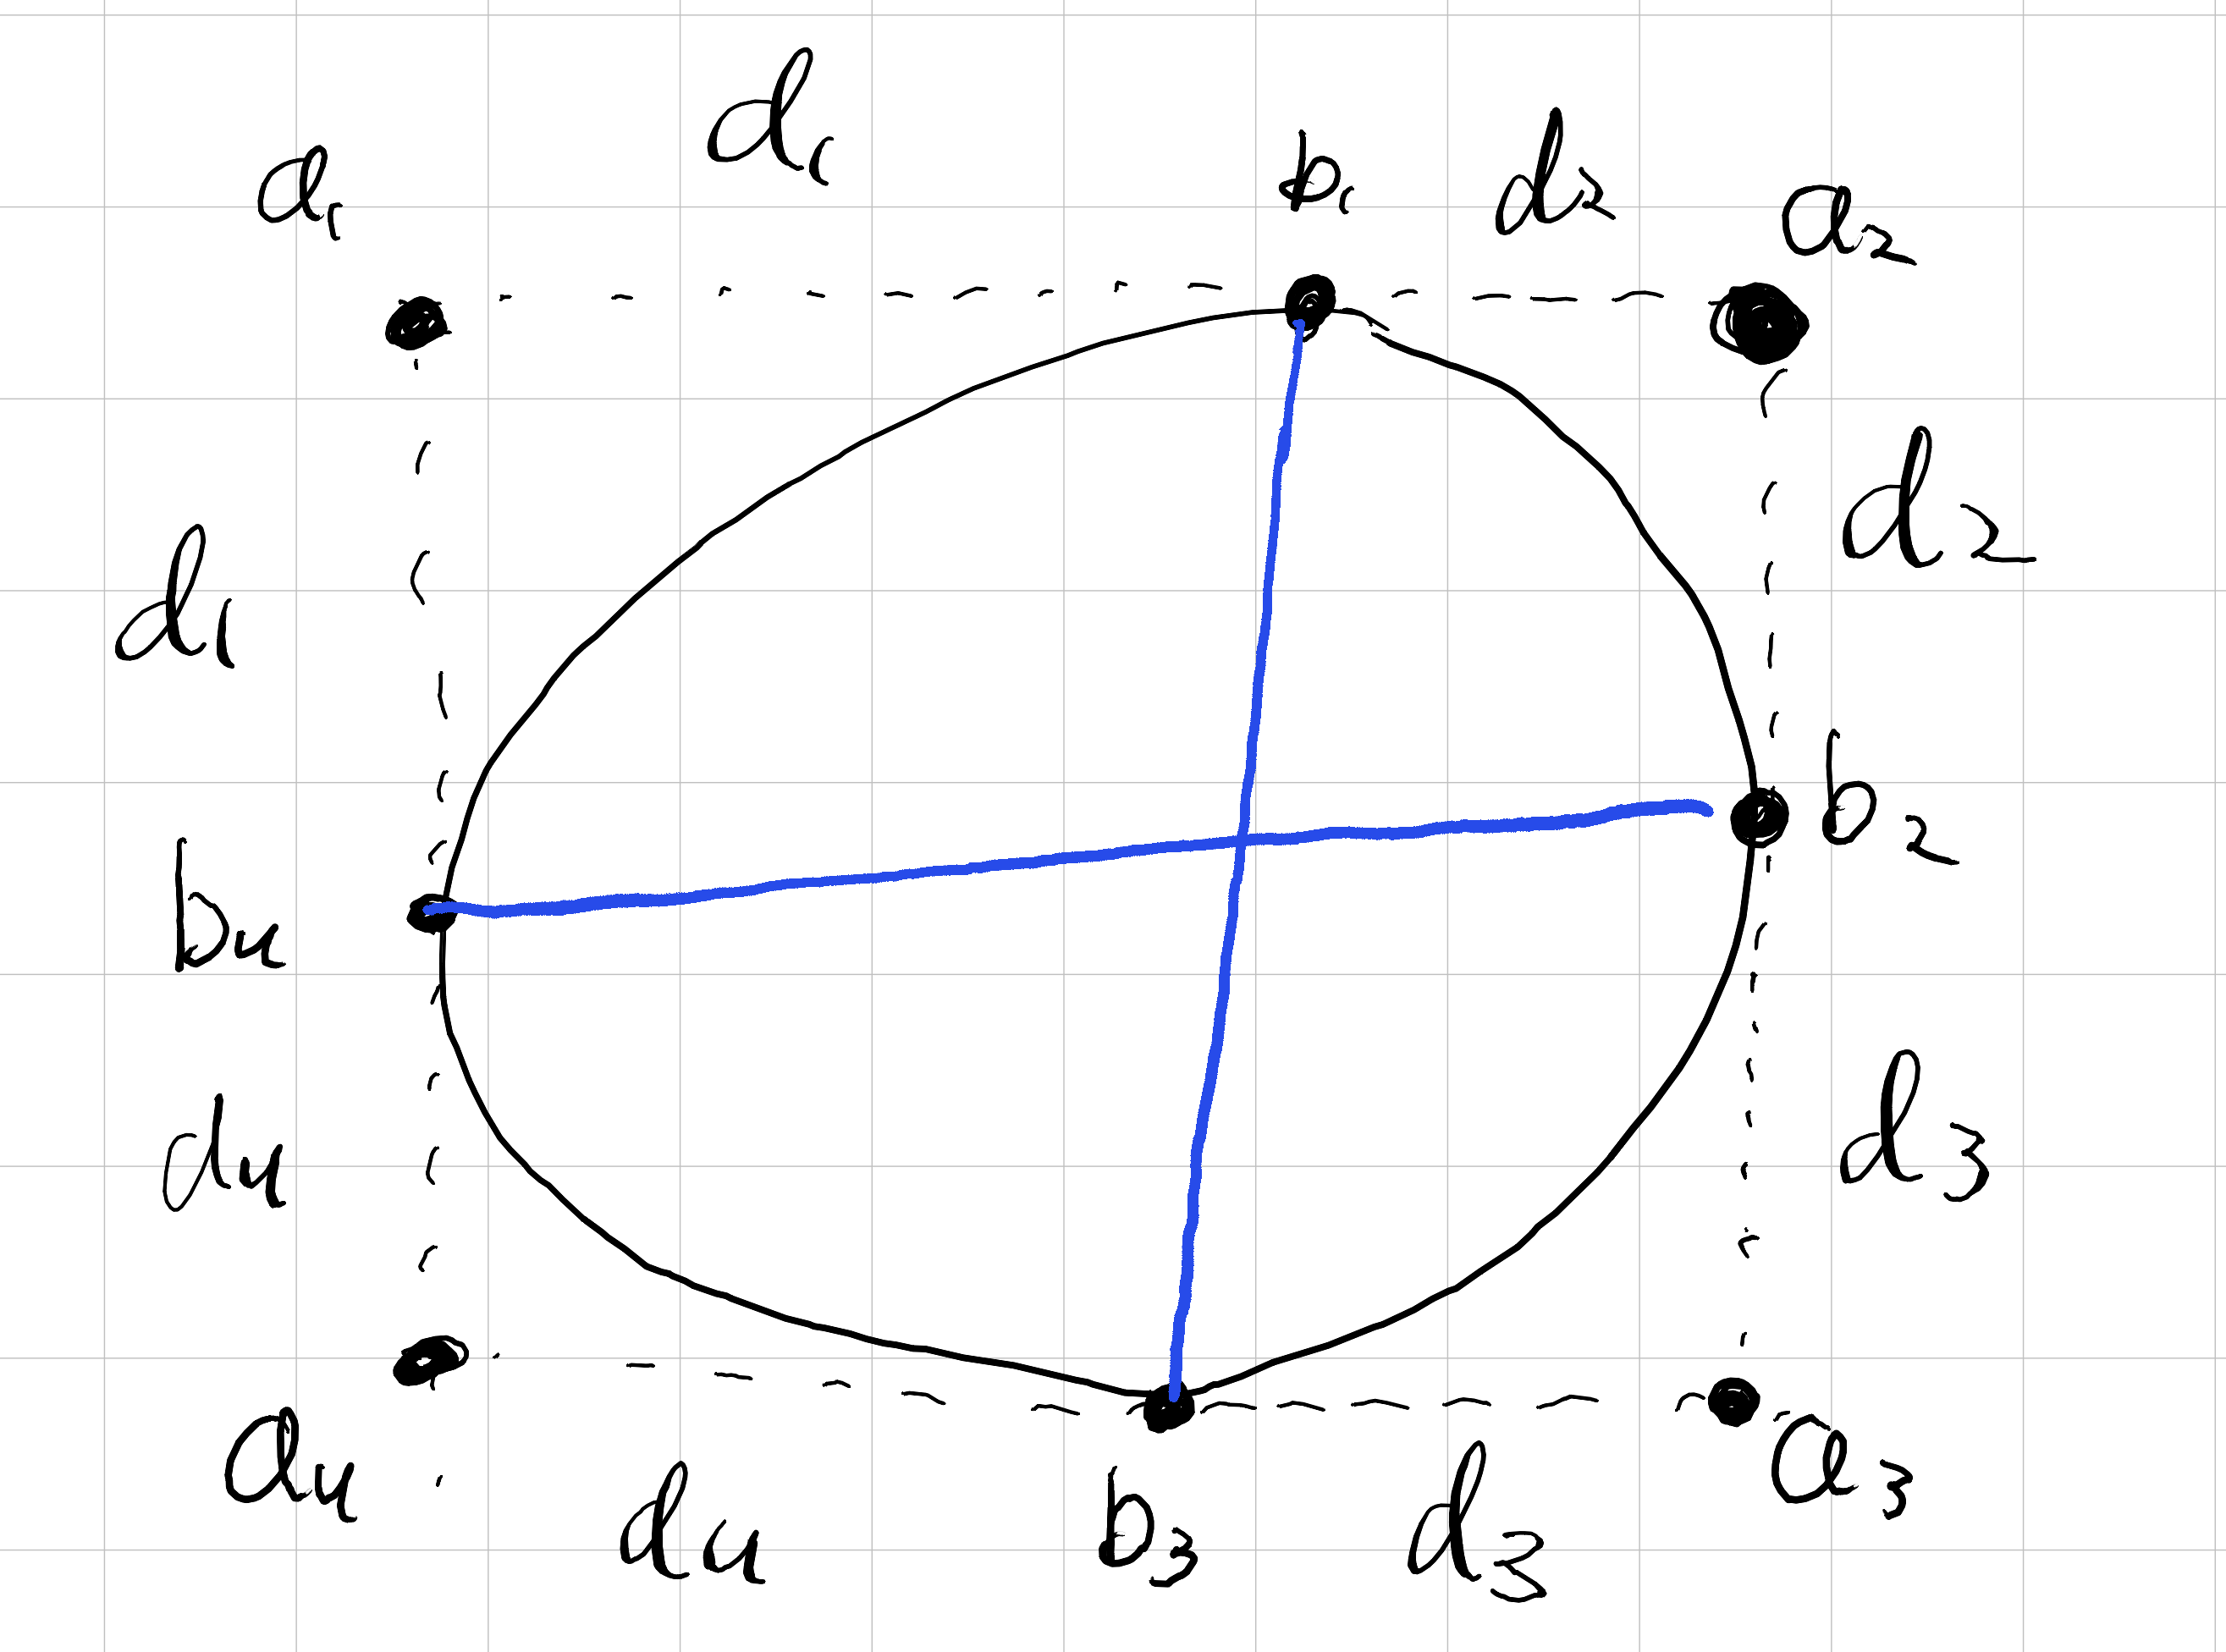
\includegraphics[width=10cm]{images/center_of_mass_problem_48.png}
  \end{center}
  We may weight $a_1,a_2,a_3,a_4$ such that $b_1$ is the center of mass of $a_1$ and $a_2$, etc. The center of mass of $a_1,\dots,a_4$ must lie on the line $b_1b_3$ and $b_2b_4$, so the lines $b_1b_3$ and $b_2b_4$ intersect.
\end{solution}

\begin{problem}[Homework Problem 53]
  What is the minimum number of breaks necessary to break an $m\times n$ chocolate bar into $mn$ pieces.
\end{problem}
\begin{solution}
  Every time we break a piece of the chocolate bar, the number of pieces increases by one. Therefore, to get $mn$ pieces from $1$ piece, we need $mn-1$ breaks.
\end{solution}
\begin{problem}[Homework Problem 54]
  Suppose that for each $x\in \R$, $f(x)$ is a finite subset of $\R\setminus \set{x}$. Show that there is an uncountable subset $S\subseteq \R$ that is disjoint from $f(S)$.
\end{problem}
\begin{solution}
  Note that $\R$ is uncountable.\newline

  Consider the set $A = \set{x \in \R | f(x) = \emptyset}$. Either $A$ is uncountable or $A$ is not. If $A$ is uncountable, then we are done.\newline

  Else, if $A$ is uncountable, we set $B = \R\setminus A$. Define $d\colon B\rightarrow \R^{+}$ to be the distance $d\left( b \right) = \dist_{f(b)}(b)$.

  We collect
  \begin{align*}
    B_n &= \set{b\in B | d(b) > \frac{1}{n}}.
  \end{align*}
  Notice that $B = \bigcup_{n\geq 1}B_n$. Since $B$ is uncountable, there exists $N$ such that $B_N$. Call this set $C$.\newline

  Partition the real numbers with width $\frac{1}{n}$. Every point in $C$ is in one of these intervals; since there are countably many intervals, there is some interval with uncountably many elements of $C$. We will define $S$ to be this subset of $C$.\newline

  For any $s\in S$, $d(s) > \frac{1}{n}$, so $f(s)$ is outside the interval, meaning $f(s)\cap S = \emptyset$.
\end{solution}

\section{Ancillary Problems}%
\begin{problem}[Ancillary Problem 1]
  Given a $n\times n$ matrix populated with the numbers $1,\dots,n^2$, show that there are two adjacent entries with difference at least $n$.
\end{problem}
\begin{solution}
  We begin by filling the grid in order --- i.e., populate by starting with $1$, then $2$, etc.
  \begin{description}[font=\normalfont\scshape,leftmargin=0pt]\itemsep=10pt
    \item[Case 1:] After filling $1,\dots,k$, there is an empty row and a full row. Now, each column has an empty cell and a filled cell. In particular, in each column there is an empty cell neighboring a filled cell. We have $n$ columns, so by the pigeonhole principle, one of these cells must receive a value at least $k+n$. Since it has a neighbor less than or equal to $k$, we are done.
    \item[Case 2:] This is the negation of $1$. So, there exists $k$ such that after filling in $1,\dots k$, each row is neither empty nor filled. Now, each row contains an empty cell and a filled cell. By the same argument as in Case 1, but substituting rows for columns, we know that by the pigeonhole principle, one of these cells must receive a value at least $k+n$. Since it has a neighbor less than or equal to $k$, we are done.
  \end{description}
\end{solution}
\begin{problem}[Ancillary Problem 2]
  Do there exist nine non-overlapping unit squares that touch central unit square $\mathbf{C}$.
\end{problem}
\begin{solution}
  Center the square $\mathbf{C}$ in a square of length $2$, and consider the square of side length $2$ as a segment of red rope.
  \begin{center}
\begin{tikzpicture}
    % Central white square with label C
    \draw[thick, black] (-0.5, -0.5) rectangle (0.5, 0.5); % white square with black border
    \node at (0, 0) {$\mathbf{C}$}; % label in the center

    % Surrounding red square with side length 2
    \draw[red, thick] (-1, -1) rectangle (1, 1); 

    % Tilted blue square
    \coordinate (corner) at (1.245, 0); % Corner of the tilted square touching the side of the central square
    \draw[blue, thick, rotate around={45:(corner)}] 
        ($(corner) + (-0.5, -0.5)$) rectangle ($(corner) + (0.5, 0.5)$); % Tilted blue square

    % Highlight the red square's border section inside the tilted square
    \begin{scope}
        \clip[rotate around={45:(corner)}] 
            ($(corner) + (-0.5, -0.5)$) rectangle ($(corner) + (0.5, 0.5)$); % Clip to the tilted square
        \draw[red, ultra thick] (-1, -1) rectangle (1, 1); % Bold red border inside the clipped area
    \end{scope}
\end{tikzpicture}
  \end{center}
  The length of the red rope contained inside a square that borders $\mathbf{C}$ is at least one; since the perimeter of the red square is $8$, it is not possible for there to be nine squares that touch $\mathbf{C}$.
\end{solution}
\end{document}
